% !Mode:: "TeX:UTF-8"
%%% Local Variables:
%%% mode: latex
%%% TeX-master: t
%%% End:

\chapter{引言}
\label{chapter:introduction}

\section{研究背景}

短波通信又称高频通信,是指使用频率范围在高频(HF)的无线电进行通信的方式\cite{董彬虹2007短波通信的现状及发展趋势}。短波通信主要利用天波电离层反射,所以无需中继站即可实现远距离通信,具有机动性强、设备成本低、对基础设施依赖小的优点,因此被广泛应用于广播、军事和抢险救灾等领域。

而同时,短波通信的缺陷也非常突出,因为受电离层变化和多径传播等因素的影响,短波通信的信道非常不稳定,导致其通信质量起伏较大,影响通信的稳定性。应对这一问题,军事中应用短波语音进行地空通信时,目前有一种解决方案:如图~\ref{fig:sys_struct}所示,在地面不同地点建立多个短波信号接收基站,接收来自空中飞机的短波语音。再将这多路信号汇总到一起,由人工选择一路质量最优的信号接入给地面指挥人员。人工选择需要的人工成本高,且稳定性和可靠性都不高,亟待使用算法代替人工。本文旨在通过对一系列算法及系统的研究,使用算法替代该方案中的人工选择步骤。

\begin{figure}
\centering
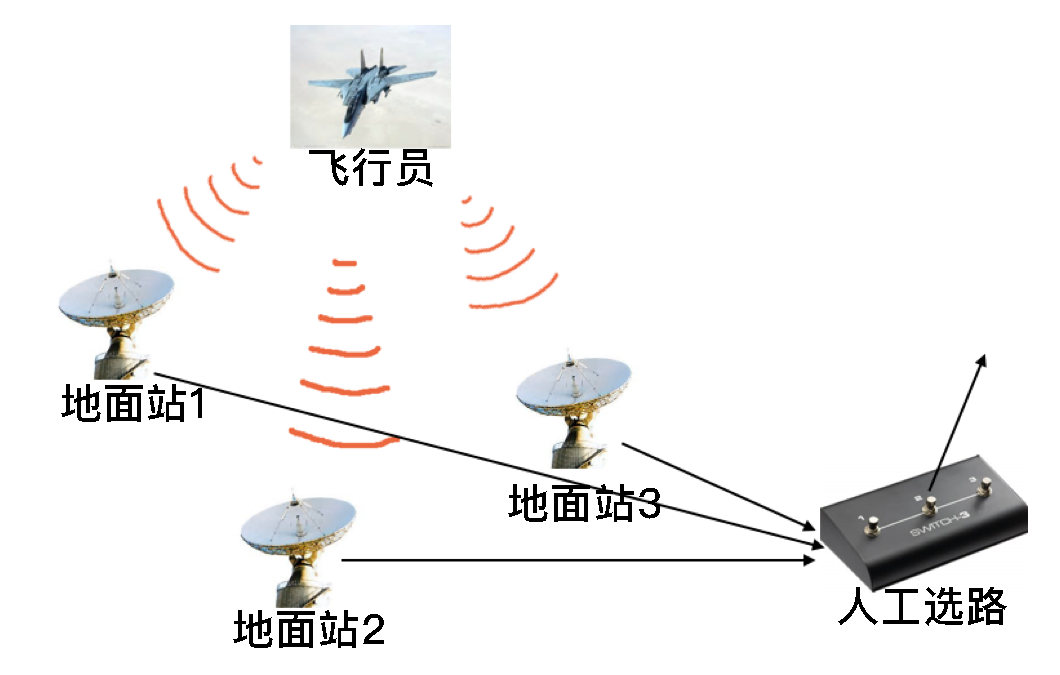
\includegraphics[width=0.8\textwidth]{sys_struct}
\caption{军事应用中的一种地空短波通信系统\label{fig:sys_struct}}
\end{figure}

\section{研究现状}

\subsection{短波通信研究现状}

\subsection{语音质量评价研究现状}

\subsection{语音增强研究现状}

\section{研究目标和研究内容}

本文的主要目标在于研究果蝇活动台分割算法和果蝇轮廓提取算法,提升算法的鲁棒性,提升果蝇行为识别算法的应用范围。本文的研究内容主要包括:
\begin{enumerate}
\item a
\item b
\item c
\end{enumerate}

\section{论文结构和内容概述}

本文剩余部分的结构如下所示:

第2章主要介绍短波语音客观质量评价算法。介绍了两种客观评价算法,一种是基于语谱图噪音模型的算法,另一种是基于人工神经网络自编码器的算法。前者根据短波语音的噪音特征设计,对于短波语音的质量评价效果非常好,但是算法针对性太强,迁移到其他领域的语音信号时,需要重新分析对应的噪音特征;而后者通过自编码器学习纯净语音信号的语谱特征,可以方便地迁移到其他领域。

第3章主要介绍多路短波语音自动选路系统。首先介绍了多路语音时间对齐算法,然后介绍了基于此算法以及第2章介绍的客观评价算法的自动选路系统。

第4张介绍了语音质量在线主观评价辅助系统,首先介绍了系统的功能和使用方法,然后介绍了系统开发和部署环境及运行原理。

第5章介绍了实验的情况。通过两组实验分别验证了第2章所提算法及第3章所提系统的实际效果,在短波语音数据集上对比了本文所提算法与两种标准质量评价算法的表现。

第6章对本文工作进行总结,并对将来可能的研究方向进行展望。

